%Dise\~no de Hardware
\section{Dise\~no de hardware} % (fold)
\label{sec:diseno_de_hardware}




Con el microcontrolador seleccionado, se procedi\'o a la etapa de dise\~no de hardware. La placa de desarrollo C8051F350 (Secci\'on \ref{sec:silicon_labs_c8051f352}) con la que se cont\'o en el laboratorio donde se trabajo, sirvi\'o de modelo para delinear el circuito esquem\'atico en la placa a desarrollar.


\subsection{Diagrama de Bloques de Hardware} % (fold)
\label{sub:diagrama_de_bloques_de_hardware}

La primera etapa de dise\~no consiste en realizar un diagrama de bloques que ilustre a grandes rasgos la organizaci\'on del circuito. Luego de esto se realiza el dise\~no esquem\'atico que consiste en llevar cada bloque a nivel de componente electr\'onico y realizar la interconexi\'on necesaria entre todos los elementos existentes para lograr el funcionamiento buscado. Los diagramas de bloque y esquem\'aticos se pueden ver en las figuras \ref{fig:bloquesHW} y \ref{fig:esquematico}. Con ayuda del software KiCad$^{\tiny{\cite{bib:kicad}}}$, se realizo el diagrama esquem\'atico y la implementaci\'on en circuito impreso correspondiente al esquem\'atico construido.

\begin{figure}[h]
  \centering
  \includegraphics[width=0.80\textwidth, height = 9cm]{bloquesHW}
  \caption{\small Diagrama de bloques del circuito a realizar}\label{fig:bloquesHW}
\end{figure}

Los bloques en la figura \ref{fig:bloquesHW} representan de forma general los distintos m\'odulos a implementar. Las entradas anal\'ogicas se introducen al sistema a trav\'es de filtros reductores del ruido. Luego, las se\~nales, ingresan al microcontrolador para ser procesadas por \'el mismo. El bloque de GPIO y contadores de eventos es simplemente un grupo de pines direccionados a distintas entradas del microcontrolador. GPIO significa ``General Purpose Input Output''( en espa\~nol, ``entrada y salida de prop\'osito general'' ). Son 4 pines que se separaron para uso general, por necesidad eventual de necesitarlos. Parte de estos GPIO son los pines contadores de eventos, por lo cual se incluyeron dentro del mismo bloque.

Es posible alimentar el sistema por medio del programador (propietario de Silicon Labs), o mediante una fuente de tension$^{\tiny{\cite{bib:lm2937}}}$ de 3,3V que se obtiene como salida de un regulador de tensi\'on, cuya entrada es de 5V. La llave selectora decide si se alimenta el sistema usando la fuente continua de 5V, o utilizando el programador.

% subsection diagrama_de_bloques_de_hardware (end)



\subsection{Diagrama Esquem\'atico} % (fold)
\label{sub:diagrama_esquematico}

La figura \ref{fig:esquematico} muestra el diagrama esquem\'atico del circuito a implementar. El microcontrolador (Secci\'on \ref{sec:silicon_labs_c8051f352}) con el que se trabaja tiene ciertos niveles de tensi\'on de operaci\'on con el que se trabaja. En principio, se alimenta con una fuente de 5V y 500mA que trabaja junto con un regulador de tensi\'on$^{\tiny{\cite{bib:lm2937}}}$ llevando la alimentaci\'on a un nivel de 3,3V. Estos 3,3V se utilizan para alimentar al microcontrolador; la tensi\'on anal\'ogica positiva del conversor; a un integrado MAX232$^{\tiny{\cite{bib:max232}}}$ que se utiliza para lograr una interfaz serial entre la UART (Secci\'on \ref{sub:interfaz_serial}) de la placa y un puerto serial de una PC; y a un led testigo de alimentaci\'on.

\begin{figure}[H]
  \centering
  \includegraphics[width=0.95\textwidth, height = 10cm]{esquem\'atico}
  \caption{\small Diagrama esquem\'atico del circuito realizado}\label{fig:esquematico}
\end{figure}

Como podemos ver, el esquem\'atico, es una proyecci\'on (a nivel electr\'onico) del diagrama de bloques. %La idea de este diagrama es que cualquier persona (que tenga conocimientos b\'asicos sobre electr\'onica) pueda entender las interconexiones, los componentes utilizados y el funcionamiento del hardware. 

% subsection diagrama_esquem\'atico (end)

\subsection{Implementaci\'on en Circuito Impreso} % (fold)
\label{sub:implementacion_en_circuito_impreso}

Una implementaci\'on en circuito impreso consiste simplemente en pasar de un diagrama esquem\'atico al despliegue f\'isico de los componentes reales en una PCB (en ingl\'es, Printed Circuit Board). Para esto, se utilizaron funcionalidades del software KiCad$^{\tiny{\cite{bib:kicad}}}$, que tambi\'en se utilizo para realizar el esquem\'atico del circuito. Una imagen del resultado del despliegue de componentes esta en la figura \ref{fig:PCB1}, as\'i con el PCB se utiliza para organizar los componentes y las interconexiones f\'isicas, de modo tal que as\'i quede en la placa impresa.

\begin{figure}[H]
  \centering
  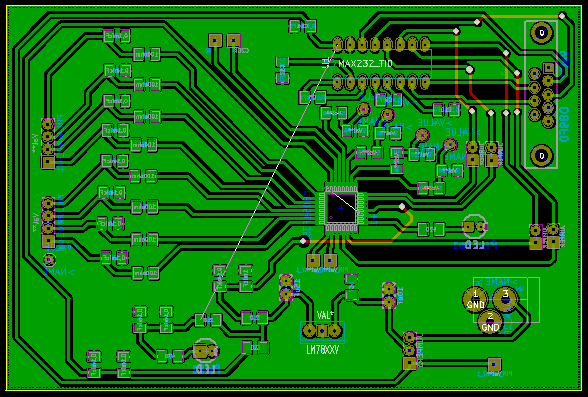
\includegraphics[width=0.95\textwidth, height = 10cm]{PCB1}
  \caption{\small Diagrama del despliegue de componentes}\label{fig:PCB1}
\end{figure}

% subsection implementaci\'on_en_circuito_impreso (end)

\subsection{Circuito anexo de programaci\'on} % (fold)
\label{sub:circuito_anexo_de_programacion}

Para programar el microcontrolador, se utiliza un programador de la marca de Silicon Labs hecho para la placa de desarrollo utilizada. Es posible usar este mismo programador en la plataforma a construir, pero es necesario armar un circuito que funcione como interfaz entre la placa del microcontrolador y el programador de la misma. El procedimiento para realizar esta placa es el mismo que se utiliz\'o para la del microcontrolador. En la figura \ref{fig:PCB2} se puede ver la figura del despliegue de componentes electr\'onicos de este circuito.

\begin{figure}[H]
  \centering
  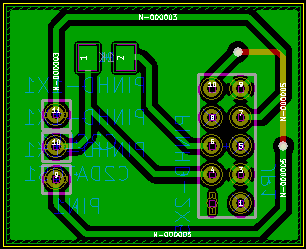
\includegraphics[width=0.20\textwidth, height = 3cm]{PCB2}
  \caption{\small Diagrama del despliegue de componentes del circuito que hace de interfaz entre el programador y la plataforma}\label{fig:PCB2}
\end{figure}

% subsection circuito_anexo_de_programaci\'on (end)

\subsection{Impresi\'on del circuito en placa de cobre} % (fold)
\label{sub:impresion_del_circuito_en_placa_de_cobre}

La impresi\'on de la placa f\'isica se implemento mas de una vez. El objetivo principal del prototipo era poder correr un programa en el microcontrolador y verificar su funcionamiento. Hubo cuatro prototipos en total. En cada una de ellas salieron a la vista distintos errores que hac\'ian necesaria una nueva impresi\'on para corregirlos.

\subsubsection{Primer prototipo} % (fold)
\label{ssub:primer_prototipo}

La primera versi\'on de la placa se puede ver en la figura \ref{fig:placa1}. En esta primera placa hubo errores de dise\~no del despliegue de componentes, ya que varias de las pistas se solapaban, y esto hubiese provocado cortocircuito entre las pistas.
\begin{figure}[h]
  \centering
  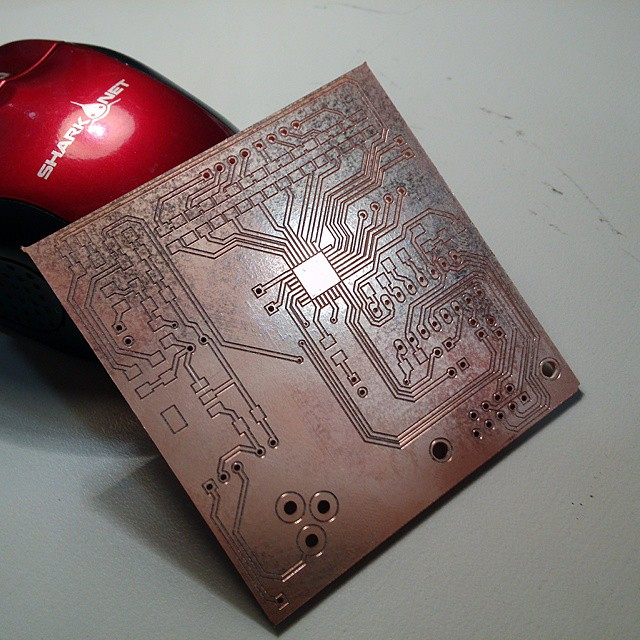
\includegraphics[width=0.60\textwidth, height = 6cm]{placa1}
  \caption{\small Fotograf\'ia del primer prototipo}\label{fig:placa1}
\end{figure}


% subsubsection primer_prototipo (end)
\subsubsection{Segundo prototipo} % (fold)
\label{ssub:segundo_prototipo}

En la segunda versi\'on se experimentaron problemas relacionados al ancho de los huecos de las patas de algunos componentes. En particular, el encapsulado del regulador de tensi\'on$^{\tiny{\cite{bib:lm2937}}}$ de 3,3V, encargado de suministrar tensi\'on al microcontrolador, no pod\'ia colocarse correctamente en la placa. Al ser una pieza tan importante, dado que sin el el microcontrolador no enciende, hubo que rehacer la placa. Una fotograf\'ia del segundo prototipo puede verse en la figura \ref{fig:placa2}.

\begin{figure}[h]
  \centering
  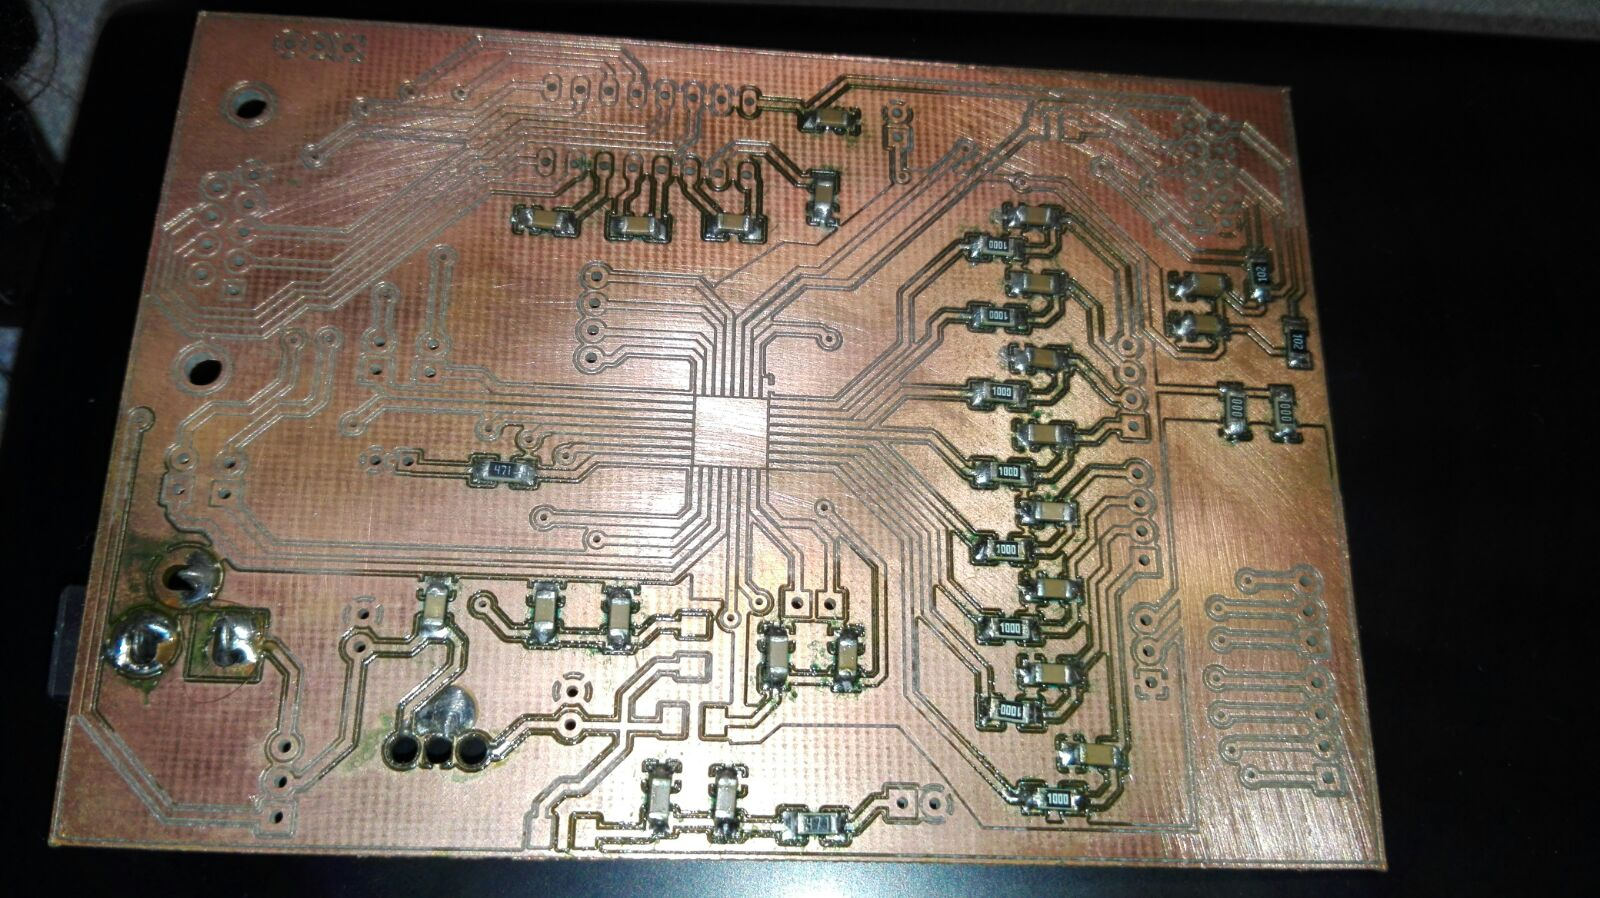
\includegraphics[width=0.60\textwidth, height = 6cm]{placa2}
  \caption{\small Fotograf\'ia del segundo prototipo}\label{fig:placa2}
\end{figure}

% subsubsection segundo_prototipo (end)

\subsubsection{Tercer prototipo} % (fold)
\label{ssub:tercer_prototipo}

La figura \ref{fig:placa3} muestra una fotograf\'ia del tercer prototipo de la placa. En esta versi\'on el problema se radico en la ficha que se utiliza para la alimentaci\'on. Hubo un cortocircuito producto de una mala soldadura, y el microcontrolador se quemo. Cuando se intento remover el chip, las pistas que conectaban al microcontrolador con el resto de los componentes se despegaron de la placa, haciendo que no nos qued\'e otra alternativa m\'as que realizar una nueva implementaci\'on. 
\begin{figure}[h]
  \centering
  \includegraphics[width=0.40\textwidth, height = 5cm]{placa3}
  \caption{\small Fotograf\'ia del tercer prototipo}\label{fig:placa3}
\end{figure}


% subsubsection tercer_prototipo (end)

\subsubsection{Cuarto prototipo} % (fold)
\label{ssub:cuarto_prototipo}

Al terminar con la ultima impresi\'on, se encontr\'o con el problema de que el microcontrolador solo lograba conectarse a al programador ocasionalmente, sin seguir un patr\'on claro. Luego de bastante tiempo buscando el problema se descubri\'o que, las resistencias que se colocan a la salida del regulador de tensi\'on eran mucho mas grandes que las que se necesitaban (se hab\'ian colocado resistencias de 470 Ohm y eran necesario colocar de 2 Ohm). Luego de detectar esto, se desoldaron las resistencias puestas y se colocaron las correctas. Luego la placa conecto correctamente al programador y a la PC. Con esto, se pudo descargar el c\'odigo realizado al mirocontrolador y ponerlo en funcionamiento. Una fotograf\'ia de la ultima implementaci\'on puede verse en la figura \ref{fig:placa4}.
\begin{figure}[h]
  \centering
  \includegraphics[width=0.40\textwidth, height = 5cm]{placa4}
  \caption{\small Fotograf\'ia del cuarto y \'ultimo prototipo realizado}\label{fig:placa4}
\end{figure}


% subsubsection cuarto_prototipo (end)
% subsection impresi\'on_del_circuito_en_placa_de_cobre (end)

% section dise\~no_de_hardware (end)